\chapter{Methodology}

{\small This chapter describes the concept of the proposed framework and the reasoning behind its design. It explains what each component does and why it was designed in the chosen way, whereas software details, model serving, and parameter values are deferred to Chapter~\ref{chap:implementation}. Section~\ref{sec:method_overview} presents the overall architecture and its central design decisions. The subsequent sections follow the flow of data through the framework: the preparation of synchronised input frames (Section~\ref{sec:method_preprocessing}), segmentation and persistent object tracking (Section~\ref{sec:method_tracking}), semantic labelling (Section~\ref{sec:method_labelling}), the fusion of semantic information with the spatial scene graph (Section~\ref{sec:method_fusion}), the representation of uncertainty (Section~\ref{sec:method_uncertainty}), and the handling of loop closures and revisited environments (Section~\ref{sec:method_loopclosure}).\par}

\section{Framework Overview}
\label{sec:method_overview}

{\small This section presents the overall structure of the proposed framework before its components are described individually in the remainder of the chapter. The structure is derived from the four aspects defined in Section~\ref{sec:goal_of_thesis}, \textit{\nameref{sec:goal_of_thesis}}, namely portability, spatial scalability, uncertainty awareness, and near-real-time operation, and from the limitations of the baseline framework~\cite{previous_rsg_thesis} identified in Section~\ref{subsec:baseline_limitations}, \textit{\nameref{subsec:baseline_limitations}}. In essence, the framework combines Hydra as a spatial backbone with a semantic pipeline that identifies objects and characterises their mobility, and joins the two through persistent object identities. Section~\ref{subsec:method_architecture}, \textit{\nameref{subsec:method_architecture}}, introduces the components and follows the flow of data between them, and Section~\ref{subsec:method_design_decisions}, \textit{\nameref{subsec:method_design_decisions}}, explains the design decisions behind this structure and relates each of them to the aspects and limitations it addresses.\par}

\subsection{Framework Architecture}
\label{subsec:method_architecture}

{\small The framework is realised as a set of ROS~2 nodes~\cite{macenski2022ros2} that exchange data through the publish-subscribe mechanism introduced in Section~2.3. It consists of three nodes developed in this thesis, the preprocessor, the Phase~1 semantic coordinator, and the scene graph fuser, and of three external software components that run as separate processes. Two of these are used entirely as provided: a Chroma vector database~\cite{chroma2026docs}, which stores the visual memory used for retrieval, and local inference servers hosting the vision-language model Qwen3.5-4B~\cite{qwen2026qwen35}, which is used for object labelling. The third, Hydra~\cite{hughes2022hydra}, serves as the spatial backbone and builds the layered 3D scene graph with its mesh, object, place, and room layers. Hydra is likewise used largely as provided; its mapping, place extraction, room detection, and loop-closure optimisation are unchanged. It was only configured with a label space of numbered slots instead of semantic classes and minimally modified to support three specific functions of the framework: objects that are segmented only after several frames can still form their own object nodes, the map can be saved and restored across sessions, and incoming frames are discarded rather than queued without limit when reconstruction falls behind. These modifications are described in the sections concerned. Because all components communicate through ROS~2 or standard network interfaces, the framework can be connected to the sensors, localisation, and mapping components of a robot in the same way as any other ROS~2 software.\par}

{\small Conceptually, the framework operates on two time scales. A per-frame path processes every incoming observation at the rate of the camera and is responsible for geometry, tracking, and mapping. An asynchronous semantic path processes individual objects rather than frames and is responsible for labels, confidence values, and mobility. The two paths are connected only through numeric slot IDs that identify persistent objects. The remainder of this subsection follows the data through both paths, and Table~\ref{tab:method_dataflow} summarises the information exchanged between the components.\par}

\begin{figure}[htbp]
	\centering
	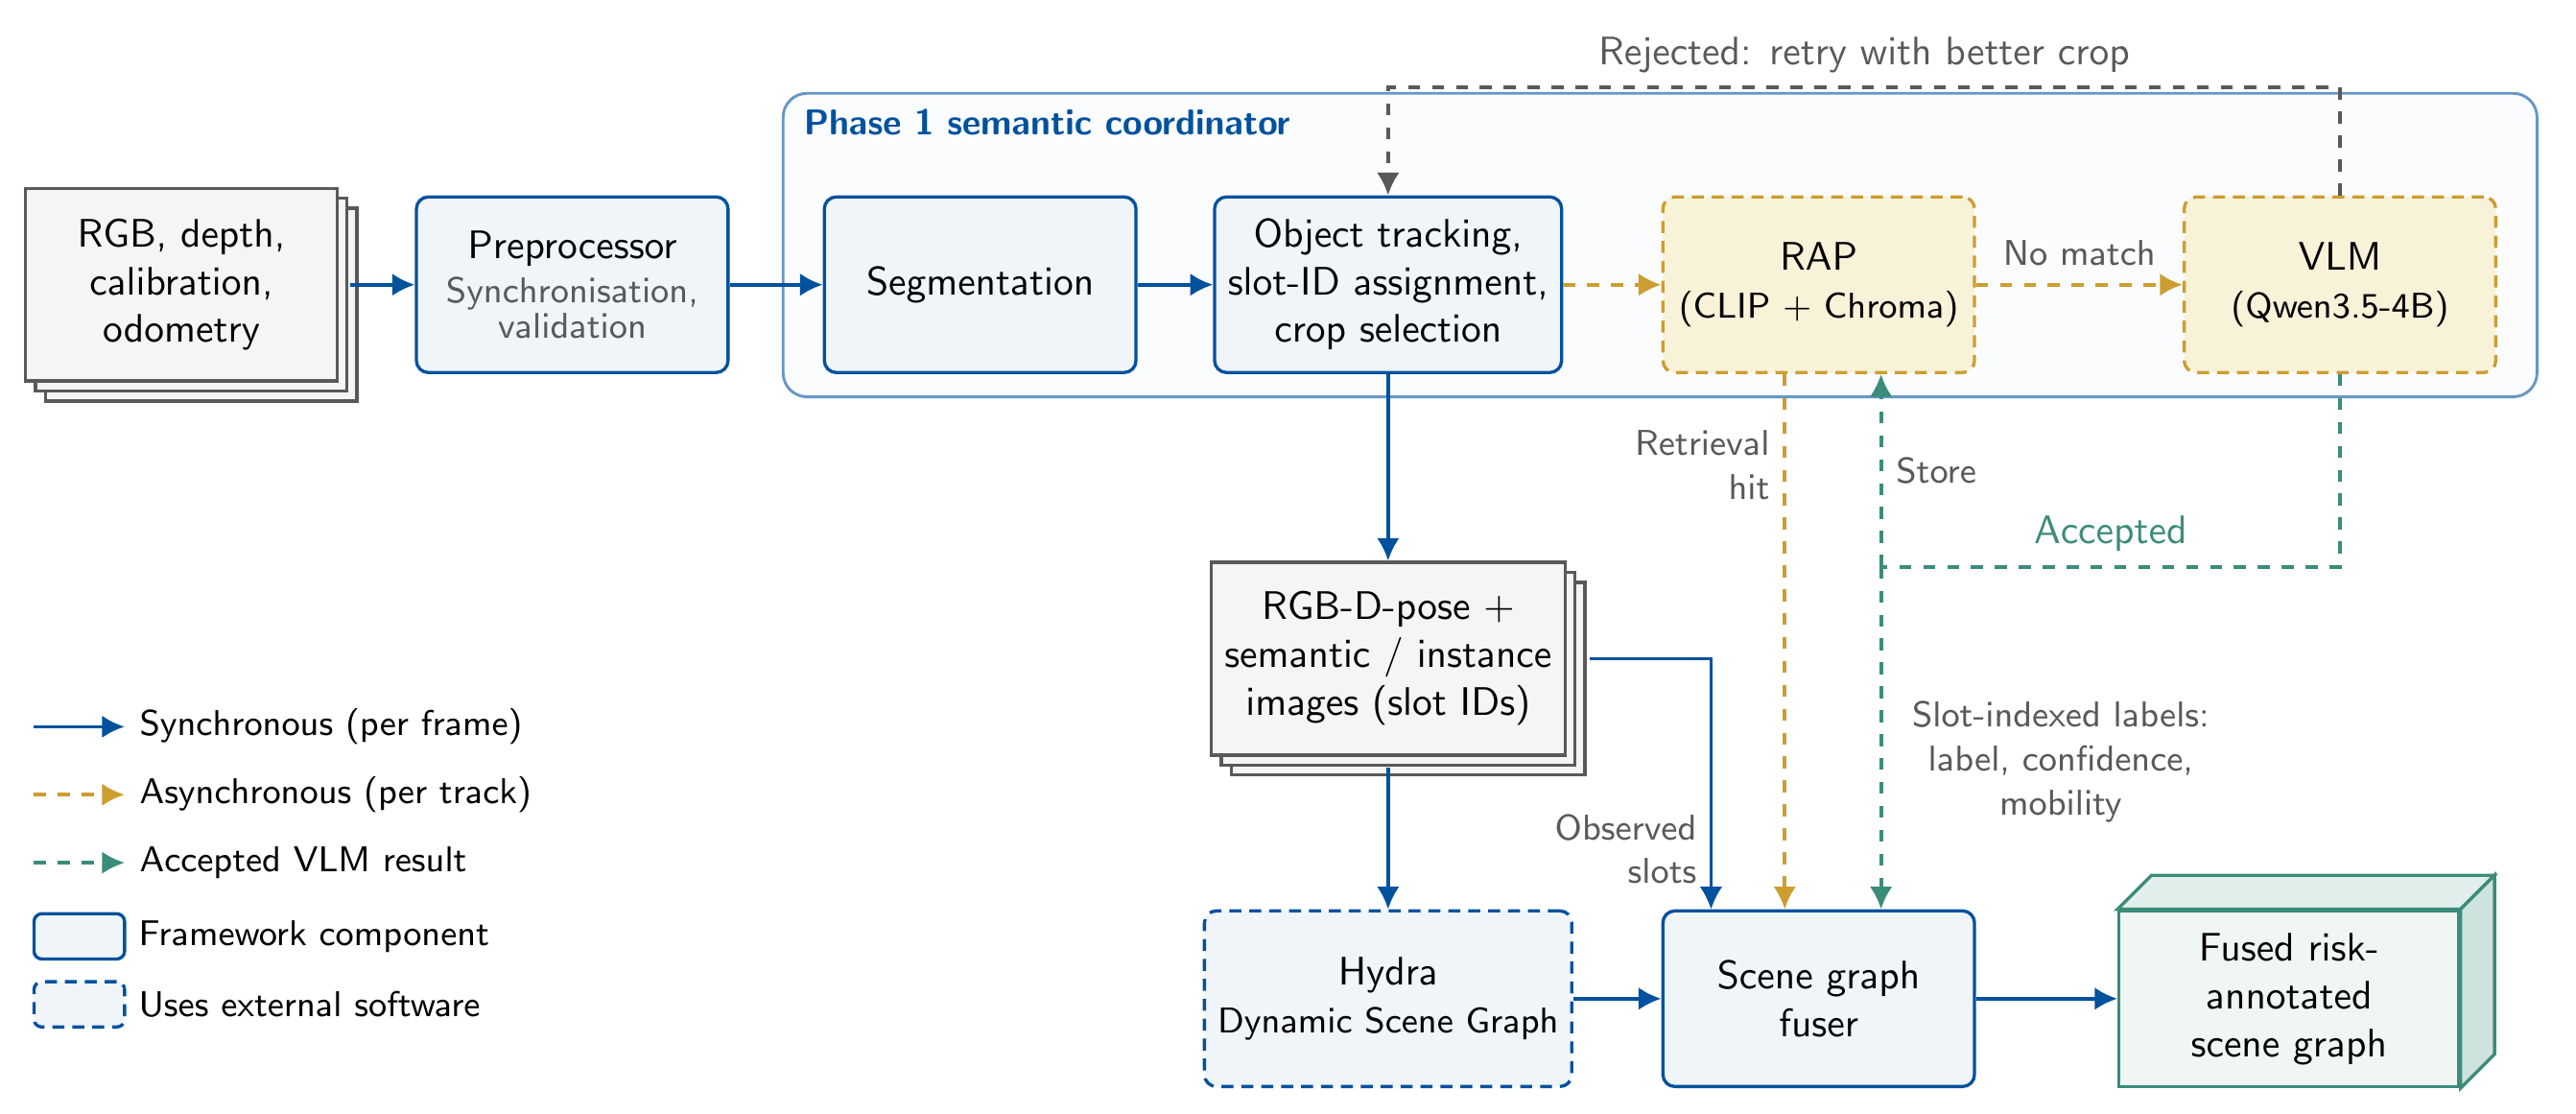
\includegraphics[width=\textwidth]{example_images/method_framework_overview.png}
	\caption{Overview of the proposed framework, showing the synchronous per-frame path (solid) and the asynchronous per-track path (dashed).}
	\label{fig:method_framework}
\end{figure}

{\small Data enters the framework at the preprocessor, which receives RGB images, aligned depth images, camera calibration, and odometry as independent timestamped streams. It associates these streams in time, rejects frames for which no consistent association exists or whose depth data is largely invalid, converts depth into metric units, and expresses the camera pose in the common map frame. The result is a single RGB-D-pose frame in which all components refer to the same instant of observation (Section~\ref{sec:method_preprocessing}). Since every downstream component consumes this representation, synchronisation is resolved once at the entry of the framework instead of repeatedly in each component.\par}

{\small On the per-frame path, the Phase~1 semantic coordinator receives each prepared frame. The colour image is segmented into class-agnostic object masks, which are back-projected with the depth image into 3D point sets with centroids and bounding boxes in the map frame. These observations are associated with persistent object tracks using primarily 3D evidence, such as the position, extent, and accumulated footprint of a track, while overlap in the image is used only as supporting evidence (Section~\ref{sec:method_tracking}). An observation that matches no existing track creates a new one. Extended structures such as floors and walls, which can span an entire room, are divided into local segments, so that a single track may be represented by several spatially bounded segments.\par}

{\small Each new track or segment is immediately assigned a slot ID from a fixed range of numbered slots. The coordinator renders the current masks into a semantic image and an instance image whose pixel values are these slot IDs and forwards them to Hydra together with the RGB-D-pose frame. Hydra is configured with this slot range as its label space instead of a fixed set of semantic classes. Since Hydra clusters mesh vertices of the same class into object nodes (Section~2.5.3), and each slot acts as its own class, every Hydra object node corresponds to exactly one track or segment. Hydra therefore receives a fully labelled input stream at the frame rate, even though no semantic label is yet known for a newly observed object, and its object layer inherits the persistent identities established by the tracker.\par}

{\small In parallel, the asynchronous semantic path assigns labels to the tracks. In contrast to the per-frame path, it operates on tracks rather than on frames. While a track is observed, the coordinator collects image crops of the object over a settling interval and retains the crop with the highest quality score, which considers, for example, the size, completeness, and sharpness of the view. Once the track is eligible, its identifier, not its crop, is placed in a queue. The crop is taken from the track only when the identifier is dequeued, so that a better view arriving in the meantime is still used. Labelling is retrieval-first: the crop is embedded with CLIP~\cite{radford2021clip} and compared with the visual memory in Chroma, following the retrieval-augmented perception principle of Section~\ref{subsec:visual_retrieval}. If a sufficiently similar reference exists, its stored label, confidence, and mobility class are reused. Otherwise, the crop is passed to the VLM in a form that emphasises the target object and suppresses its surroundings, and the model returns a structured result consisting of a label, a confidence value, and a mobility class (Section~\ref{sec:method_labelling}). Results that are malformed or fall below a confidence threshold are rejected, and the track waits for a better crop before it is retried a limited number of times. Every accepted VLM result is written back into the memory together with the crop that produced it. Labelling results are published as slot-indexed events. In addition, the coordinator publishes for every frame which slots were observed, which provides the evidence for the presence model of the fuser.\par}

{\small Two properties of this path are essential. First, the VLM only ever receives image crops of a single object; it never receives the full scene graph or a cutout of it, and it is never asked to generate graph structure. Second, retrieval and labelling lie entirely off the per-frame critical path. Their results arrive later and in arbitrary order, which affects only when semantic information becomes available, not whether segmentation, tracking, and mapping can proceed.\par}

{\small The two paths are brought together in the scene graph fuser, which subscribes to Hydra's Dynamic Scene Graph and to the events of the semantic path. Incoming events only update a cache indexed by slot ID; at a bounded rate, the fuser applies the cached labels, confidence values, and mobility classes to every Hydra object node that carries the corresponding slot (Section~\ref{sec:method_fusion}). Labels that arrive long after an object was first mapped are thus applied as soon as they are available. The fuser further completes the relational structure of the graph. Contact between objects and the relation between an object and the local segments of an extended structure are derived from the 3D bounding boxes, room and place membership are taken from Hydra's layers, and missing object-to-place links are added only where a geometric check against the reconstructed mesh confirms them. For every slot, the fuser maintains a presence confidence that is reset by observations and decays while the object is unobserved, at a rate that depends on its mobility class (Section~\ref{sec:method_uncertainty}). The result is published as the fused risk-annotated scene graph, which can be visualised in RViz and consumed by downstream risk assessment.\par}

{\small Two further mechanisms keep the scene graph consistent over time. When the localisation back-end corrects accumulated drift, the transform between the map frame and the odometry frame changes. Hydra corrects its own scene graph through its deformation-based optimisation (Section~2.5.4). The coordinator detects such corrections, shifts its cached object geometry accordingly, and merges tracks that were created twice for the same object around the closure, so that the tracker remains consistent with Hydra's corrected map. In addition, both the tracker state and Hydra's map can be saved at the end of a session and restored at the beginning of the next. Re-observed objects are then associated with their earlier tracks in Phase~1 and merged with their restored object nodes in Hydra, so that an environment that is revisited in a later session is not mapped a second time (Section~\ref{sec:method_loopclosure}).\par}

\subsection{Central Design Decisions}
\label{subsec:method_design_decisions}

{\small The architecture described above is the result of a small number of design choices, which are best understood as answers to a single underlying problem. The framework has to combine two kinds of processing that operate on very different time scales. Spatial mapping must keep pace with the camera, since a map that lags behind the robot is of little use for assessing the current situation. Open-vocabulary identification, on the other hand, relies on a vision-language model whose inference takes far longer than the interval between two frames. The baseline framework coupled both in a single per-frame loop, so that the slowest component determined the update rate of the entire scene graph. The design choices discussed in this subsection all follow from the aim of separating these two time scales without losing the connection between them.\par}

{\small The starting point was the question of where the spatial representation should come from. The baseline maintained its own frame-based graph, which had neither a common map frame nor loop closure. Extending this graph with the required spatial capabilities would have meant re-implementing incremental mapping, a mesh-grounded object layer, places and rooms derived from free-space topology, and loop-closure correction, all of which Hydra already provides in a real-time architecture that has been evaluated on robotic data~\cite{hughes2022hydra}. Other spatial scene graph systems were less suitable as a foundation: SceneGraphFusion~\cite{wu2021scenegraphfusion} is restricted to a closed set of classes, and ConceptGraphs~\cite{gu2024conceptgraphs} applies foundation models to every observation, which is precisely the coupling that limits the update rate. Hydra was therefore adopted as the spatial backbone and deliberately kept close to its original form. Its mapping and optimisation algorithms are used unchanged, and the few modifications are confined to what the framework strictly needs. This lets the work of this thesis concentrate on what Hydra does not offer, namely open-vocabulary semantics, mobility, and uncertainty, and keeps the framework compatible with future versions of Hydra.\par}

{\small Adopting Hydra, however, brings one of its assumptions with it. Hydra forms object nodes by clustering mesh vertices that share a semantic label, and therefore expects every pixel to be labelled before it is integrated into the map. Supplying real class labels would have required either a closed set of classes, which contradicts open-vocabulary identification, or holding back Hydra's input until the vision-language model has answered, which reintroduces the coupling that the framework is meant to remove. The slot IDs resolve this conflict. Instead of a label, each pixel carries the identifier of the persistent track it belongs to, which is available immediately after tracking. Hydra can thus cluster objects exactly as designed, at its native rate, while never seeing a semantic label at all. The meaning of each slot is supplied later and independently, and because a slot never changes once assigned, the object nodes in Hydra's map inherit the persistent identities established by the tracker.\par}

{\small Once geometry no longer depends on semantics, semantic processing is free to run at its own pace. Labelling is therefore organised around tracks rather than frames and is executed from bounded queues that are decoupled from the camera. A slow or temporarily unavailable inference server can delay labels, but it cannot stall segmentation, tracking, or mapping, and when the queue is full, pending work is deferred rather than allowed to block the pipeline. A useful side effect is that the crop of an object is only chosen when its track is actually processed, so that time spent waiting can produce a better view of the object. The cost of this arrangement is that a newly observed object appears in the map before it has a label. This is acceptable, since such objects are explicitly marked as unlabelled rather than misrepresented, and since they are already geometrically present and can be treated as obstacles by downstream components.\par}

{\small Decoupling makes the cost of the vision-language model tolerable, but it does not reduce it, nor does it make the output of the model any more reliable. Both concerns are addressed in how labelling itself is organised. In a typical indoor environment, the same objects are observed again and again, and many objects resemble others that have already been labelled. Consulting a visual memory before the model resolves such cases at a small fraction of the cost, and because every accepted result is added to that memory, the framework relies on the model less the longer it operates. When the model is needed, it is given a single-object crop and must answer in a fixed format with a small number of fields, each of which is checked before the result is accepted. Malformed or low-confidence answers are rejected instead of being written into the graph. This replaces the free-form graph updates of the baseline, whose errors passed directly into the scene representation, with an output that can be validated while remaining open-vocabulary. Since an incorrect entry in the memory would be propagated to every similar object, only validated results are stored there.\par}

{\small The last choice concerns what happens when semantic information reaches the scene graph. Because labels arrive late and objects move out of view, the fused graph has to express how much it knows about each object rather than present every entry as equally certain. The fuser therefore never alters Hydra's scene graph and attaches all semantic and confidence information as derived metadata, so that the spatial structure remains exactly as Hydra built it. Relationships between objects are derived from their 3D geometry rather than generated by the model, which makes them properties of the scene instead of impressions that depend on the viewpoint, such as \textit{in front of} or \textit{behind}. This also reduces the load on the vision-language model compared with the baseline, in which the model had to infer all spatial relationships of the visible scene in every inference step, in addition to identifying the objects themselves. In the proposed framework, the model is only asked to identify a single object, which keeps both its input and its output small. Where the baseline deleted objects once their appearance score fell below a threshold, the proposed framework expresses doubt about an object's continued presence through a confidence value that is reset whenever the object is observed and decays while it is not. The rate of decay follows the mobility of the object: the confidence of a static object that is out of view decreases slowly, whereas the confidence for humans, animals, and mobile robots decreases considerably faster, reflecting that they have probably moved. The decay rates are configurable and can be adapted to the dynamics of the environment. Only tracks confirmed as dynamic are eventually withdrawn from the fused output, and the underlying map is never pruned. Downstream risk assessment can thus distinguish objects whose state is well known from those whose state has become uncertain, which is the information that the appearance score of the baseline could not provide.\par}

{\small Taken together, these choices assign each part of the problem to the component best suited to it. Hydra provides spatial consistency and scalability, the slot IDs connect geometry and semantics without making either wait for the other, asynchronous and retrieval-first labelling keep the cost of open-vocabulary identification compatible with near-real-time operation, and confidence-annotated fusion makes the remaining uncertainty explicit. Because all components communicate through ROS~2 or standard network interfaces, the same structure can be integrated into a robotic system without changes to the components themselves.\par}

























% ---------------------------------------------------------------------------
% Section 3.2 -- replaces the old sections "Hardware Setup and Input Data
% Preparation", "Data Preprocessing" and the empty "Pre-Processing" in
% chapters/Methodology.tex.
% NOTE: copy the old "Hardware Setup and Input Data Preparation" text into a
% separate file (for Chapter 4, Implementation) BEFORE deleting it.
% ---------------------------------------------------------------------------

\section{Data Acquisition and Preprocessing}
\label{sec:method_preprocessing}

{\small The components described in Section~\ref{sec:method_overview} require each observation to combine visual, geometric, and pose information that refers to the same instant. The sensor data, however, consists of independent timestamped streams of colour images, depth images, odometry, and camera calibration, which are produced at different rates. The preprocessing stage combines these streams into a single \emph{prepared RGB-D-pose frame}, which constitutes the input contract of the framework. Since every downstream component consumes this frame, synchronisation is resolved once at the entry of the framework rather than separately in each component. The stage processes each observation as a sequence of steps, illustrated in Figure~\ref{fig:preprocessing_flow}, in which a frame is passed on only if it satisfies both temporal and geometric consistency and is rejected otherwise.\par}

{\small
\begin{figure}[htbp]
\centering
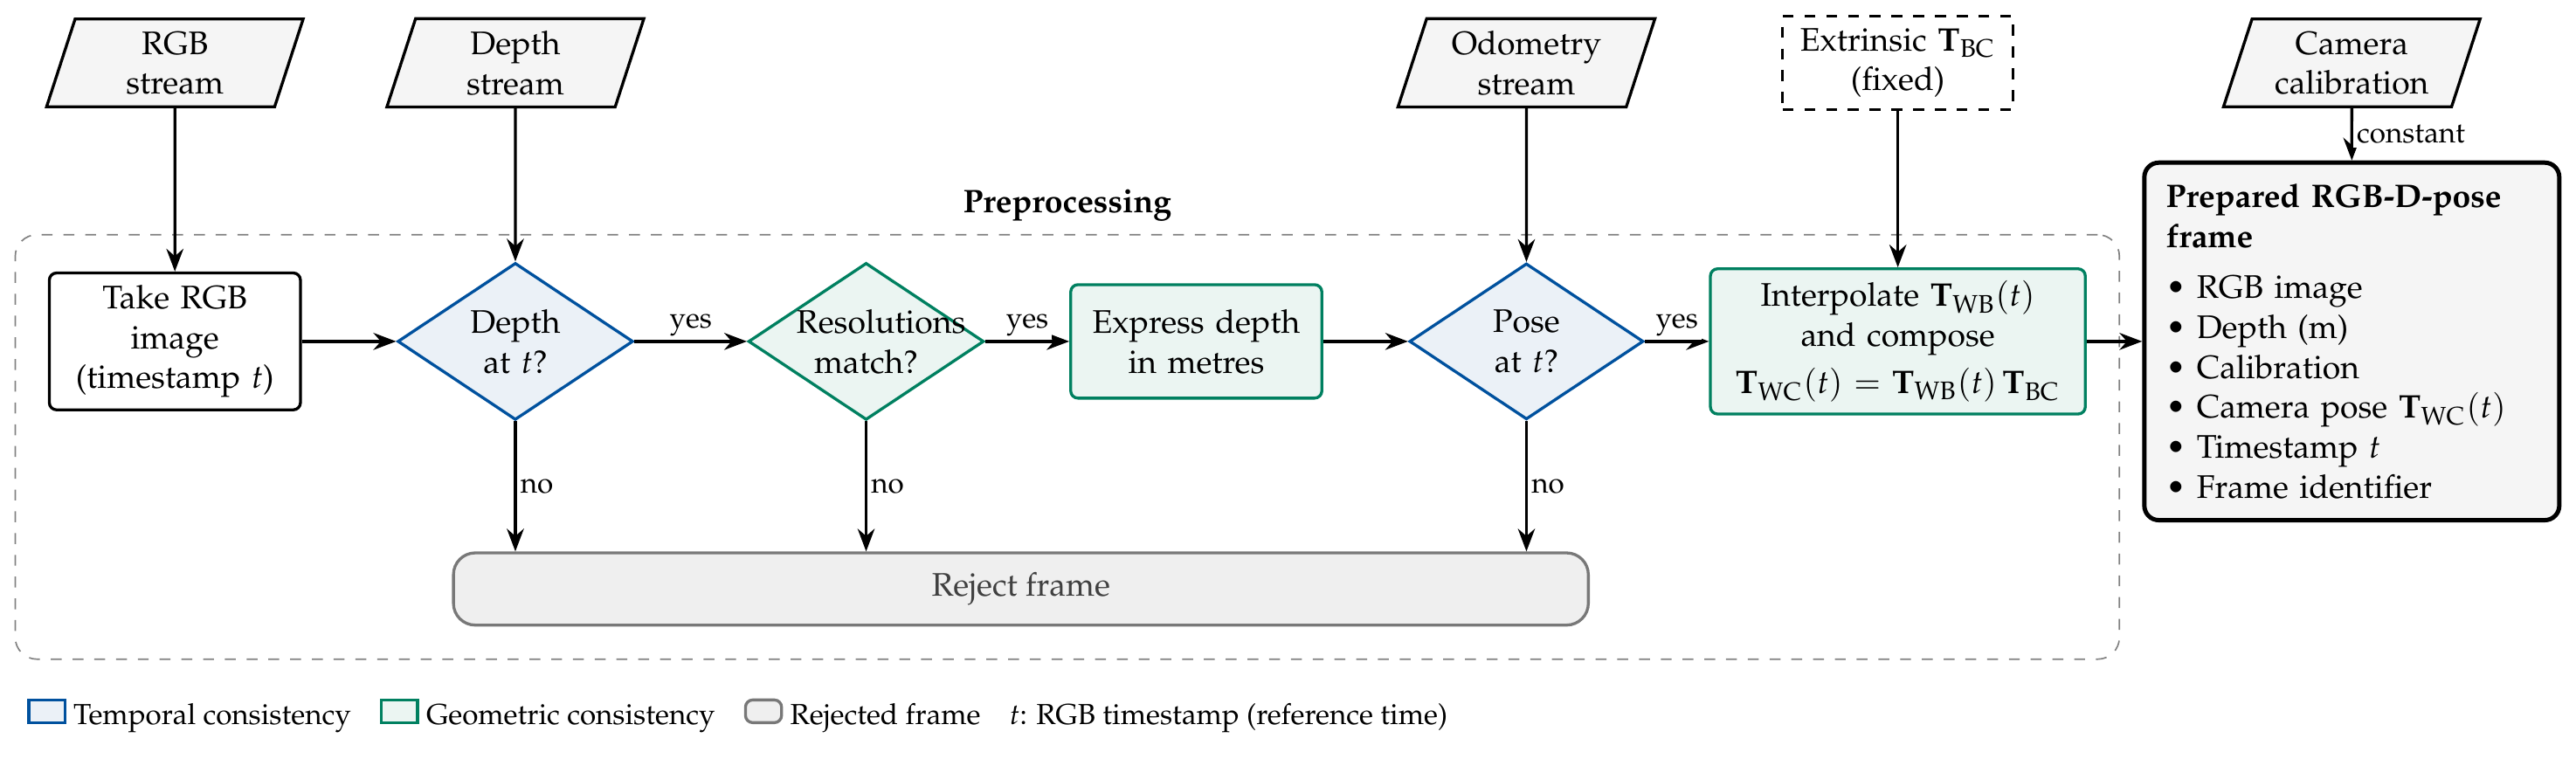
\includegraphics[width=\textwidth]{example_images/preprocessing_flow.png}
\caption{Preprocessing of the input streams into a prepared RGB-D-pose frame.}
\label{fig:preprocessing_flow}
\end{figure}
\par}

{\small Each frame is anchored to an RGB image, whose timestamp $t$ serves as the reference time for all subsequent steps. The first step checks whether a depth image with approximately the same timestamp is available. If no such depth image exists, the frame is rejected, since the colour image cannot be related to the 3D structure of the scene. The second step checks geometric consistency between the two images, which must have identical resolution, so that each colour pixel corresponds to the same depth pixel and a segmentation mask computed on the RGB image can be lifted directly to 3D. A frame that violates this condition is likewise rejected. The depth image is then expressed in metric units, which are used throughout the framework; sources that provide depth in other units are converted at this stage. Depth values are, however, not filtered here, since range filtering is performed in Phase~1 (Section~\ref{sec:method_tracking}), where depth is first used.\par}

{\small The third step checks whether the pose of the robot at time $t$ can be determined from the odometry. Since odometry is generally not sampled at the same instants as the camera, the base pose $\mathbf{T}_{\mathrm{WB}}(t)$ is interpolated to the RGB timestamp, which reduces the geometric error that would otherwise arise when an image captured during motion is projected with a pose from a slightly different time. If no sufficiently close odometry is available, the frame is rejected. This reflects a deliberate design choice: Hydra~\cite{hughes2022hydra} integrates every received frame into a persistent map, so discarding an inconsistent frame is preferable to integrating geometrically inconsistent data. Since the odometry describes the pose of the robot base rather than that of the camera, the camera pose is obtained by composing the interpolated base pose with the fixed transform from the robot base to the camera:
\begin{equation}
  \mathbf{T}_{\mathrm{WC}}(t) = \mathbf{T}_{\mathrm{WB}}(t)\,\mathbf{T}_{\mathrm{BC}},
  \label{eq:camera_pose}
\end{equation}
where $\mathbf{T}_{\mathrm{WB}}(t) \in SE(3)$ denotes the pose of the robot base in the world frame at time~$t$, $\mathbf{T}_{\mathrm{BC}} \in SE(3)$ denotes the calibrated extrinsic transform from the robot base to the camera, and $\mathbf{T}_{\mathrm{WC}}(t)$ is the resulting camera pose. The world frame is the fixed reference frame of the odometry source. Since $\mathbf{T}_{\mathrm{BC}}$ is constant, the camera is assumed to be rigidly mounted on the robot.\par}

{\small Finally, a frame that has passed all checks is assembled into the prepared RGB-D-pose frame. It contains the RGB image, the depth image in metres, the intrinsic camera calibration, the camera pose $\mathbf{T}_{\mathrm{WC}}(t)$, the timestamp $t$, and a unique frame identifier. The calibration is not part of the sequential checks, as the intrinsic parameters remain constant during operation and are attached to every frame.\par}

{\small The preprocessing stage is kept intentionally minimal, as it lies on the per-frame path of the framework and any latency it introduces delays all subsequent components. It therefore performs only the operations needed to establish the consistency conditions described above. Furthermore, the method is independent of the data source: applying it to the simulated uHumans2 dataset~\cite{rosinol2021kimera} or the real-world OpenLORIS-Scene dataset~\cite{shi2020openloris} changes only the sensor-specific parameters, such as the base-to-camera transform and the depth unit, while the sequence of checks and Equation~\eqref{eq:camera_pose} remain unchanged .\par}


























\section{Object Segmentation and Persistent Tracking}
\label{sec:method_tracking}
{\small
Class-agnostic segmentation of the frames prepared in Section~\ref{sec:method_preprocessing} yields an unordered set of masks without identity. For each mask, the framework must decide whether it shows a new physical object or a further observation of a known one, and it must maintain a persistent three-dimensional estimate of every object. The two association errors identified in Section~\ref{subsec:data_association} have strongly asymmetric consequences here. If two objects are merged into one track, its geometry describes neither of them and the crop passed to the vision-language model shows parts of both, so the label is wrong for both; since label and geometry belong to the track as a whole, this cannot be repaired downstream. If one object is fragmented into several tracks, the representation becomes redundant, but each fragment remains correct and can, in principle, be merged later. The method therefore follows a single design principle: whenever the evidence is ambiguous, fragmentation is preferred over over-merging.
\par}

\subsection{Object Proposals and 3D Observations}
\label{subsec:method_proposals}
{\small
Object proposals are generated by a promptable model of the Segment Anything family~\cite{kirillov2023segmentanything}, prompted with a regular grid of foreground points. A common interface returns a set of class-agnostic masks, so the remainder of the method is independent of the model behind it. Two interchangeable models are supported: the original SAM with a ViT-B encoder and NanoSAM (Section~\ref{sec:nanosam}), which has a considerably lower latency on embedded hardware but reduced accuracy, particularly for small objects~\cite{nanosam2023}. SAM uses its own automatic mask generation, whereas for NanoSAM the equivalent post-processing is realised as a wrapper (Section~\ref{subsec:nanosam_limitations}). In both cases, duplicate masks from neighbouring prompts are removed by non-maximum suppression, and implausibly small masks are discarded, as they rarely represent complete objects and provide too few depth measurements. To bound the cost of all subsequent stages, the number of proposals per frame is limited, retaining the masks with the highest predicted quality. Since the choice of model trades proposal quality against update rate, it is determined experimentally in Chapter~\ref{chap:experiments}. The result is a set of masks $\mathcal{M}_t = \{m_1, \dots, m_N\}$ for frame $t$.

Each mask is converted into a three-dimensional observation. Depth is taken only from the largest connected region of the mask, because masks often contain detached fragments and boundary regions whose depth belongs to the background. A pixel $(u, v)$ with valid depth $d$ is back-projected with the pinhole model and transformed into the map frame using the camera pose of Equation~\ref{eq:camera_pose}:
\begin{equation}
	\mathbf{p}^{c} = d \begin{bmatrix} (u - c_x)/f_x \\ (v - c_y)/f_y \\ 1 \end{bmatrix},
	\qquad
	\mathbf{p}^{m} = \mathbf{R}^{m}_{c}\,\mathbf{p}^{c} + \mathbf{t}^{m}_{c},
	\label{eq:backprojection}
\end{equation}
where $f_x$, $f_y$, $c_x$ and $c_y$ are the focal lengths and principal point, and $(\mathbf{R}^{m}_{c}, \mathbf{t}^{m}_{c})$ is the transformation from the camera to the map frame. The resulting point set $\mathcal{P}_i$ is summarised as an observation $o_i = (\mathcal{P}_i, \mathbf{c}_i, \mathcal{B}_i, \mathbf{b}_i)$ with the axis-aligned three-dimensional bounding box $\mathcal{B}_i$ of the points in the map frame, its centre $\mathbf{c}_i$, which serves as the centroid of the observation, and the two-dimensional bounding box $\mathbf{b}_i$ of the mask in image coordinates. Since thin structures such as floors, ceilings and walls yield boxes of almost zero thickness, for which a volumetric overlap is not meaningful, every box dimension below a minimum thickness is padded to that thickness before $\mathbf{c}_i$ and the volume are computed. The three-dimensional quantities provide viewpoint-invariant evidence for association, while $\mathbf{b}_i$ is used for the image-space comparison and for extracting the object crop. A mask without reliable geometry, for instance because most of its depth values are invalid, is discarded for the current frame, and no observation, crop or track is created from it. The object is not ignored: it is expected to be observed again with meaningful depth as the robot moves, and is tracked then. Discarding the mask only keeps inaccurate data out of the persistent representation; moreover, an observation without geometry could not be associated by the three-dimensional evidence and would only open short-lived tracks.

Depth values outside a valid sensing range are excluded during back-projection, completing the filtering deferred in Section~\ref{sec:method_preprocessing}. This serves two purposes. First, depth accuracy decreases with distance: for a stereo camera, the error grows approximately quadratically, $\delta z \approx z^{2}\,\delta_{d} / (f\,b)$, with depth $z$, focal length $f$, baseline $b$ and disparity error $\delta_{d}$~\cite{keselman2017realsense}. Distant points therefore yield noisy centroids and inflated boxes, which weaken the association cues and, through the accumulated extent (Section~\ref{subsec:method_track_state}), could permanently distort a track. Measurements below the sensor's minimum operating distance are excluded for the same reason. Second, the restriction limits the computational cost per frame, since masks of distant objects are discarded before association, crop selection and labelling, so that the expensive vision-language model inference is applied only to objects near the robot. Distant objects are observed again once they enter the valid range, and nearby objects are generally the most relevant for immediate risk assessment.
\par}

\subsection{Evidence-Based Association}
\label{subsec:method_association}
{\small
Association is performed primarily in three dimensions, because the position and extent of a static object in the map frame are approximately constant across viewpoints, whereas its image appearance is not (Section~\ref{subsec:data_association}). Fusion++, in contrast, relies on a single image-space overlap criterion~\cite{mccormac2018fusion}. An observation $o$ is compared only with candidate tracks $\tau$ in its spatial neighbourhood, which are retrieved by a grid search over a uniform grid in the ground plane: each track is registered in the cells covered by its accumulated extent and by its centroid, and the candidates are the tracks registered in the cells covered by the observation's footprint or lying within the centroid acceptance radius. Since a track outside these cells can pass neither the overlap nor the centroid test, it cannot satisfy the acceptance condition below, so the grid search reduces the cost per observation without changing the association result. The evidence is organised hierarchically: the three-dimensional overlap is the primary evidence, while centroid distance and image overlap are secondary evidence that is consulted only when the overlap is not conclusive.

The primary evidence is the volumetric overlap between the observation's bounding box and the accumulated extent of the track, which reflects that a static object occupies the same region of the map from any viewpoint. The accumulated extent is used because successive views often capture different parts of an object, and overlap is required on both horizontal axes, so that boxes that merely touch do not count. Two levels are distinguished. A partial overlap shows a shared region but is ambiguous, since adjacent objects also overlap partially. A near-complete inclusion of the observation in the track's extent, referred to as containment, is the expected outcome of a re-observation, especially for large objects such as floors and walls that are seen only in part. In addition, a height test requires only the vertical extents to overlap or to be separated by at most a small gap, irrespective of horizontal position. A volumetric overlap therefore implies height compatibility, but not vice versa, since boxes at the same height may lie side by side.

The secondary evidence resolves the ambiguity of a partial overlap. The centroid distance separates objects whose boxes intersect but whose centres lie apart. It is mapped to a similarity by a Gaussian kernel whose width scales with object size, because the centroid of a large, partially observed object shifts more between views. The image overlap between $\mathbf{b}$ and the box of the track's last observation is independent of depth and pose errors and strongly indicates continuity between consecutive frames, but its value decreases quickly as the viewpoint changes.

Each test $k$ yields a similarity $\sigma_k(o, \tau) \in [0, 1]$ and a binary verdict $\pi_k(o, \tau) \in \{0, 1\}$. With $\pi_{\mathrm{con}}$, $\pi_{\mathrm{ov}}$, $\pi_{\mathrm{h}}$, $\pi_{\mathrm{cen}}$ and $\pi_{\mathrm{img}}$ denoting the verdicts for containment, partial overlap, height, centroid distance and image overlap, a match in association mode $\mu$ is accepted if
\begin{equation}
	\begin{aligned}
	&s^{(\mu)}(o, \tau) = \frac{\sum_{k} w_k^{(\mu)}\, \sigma_k(o, \tau)}{\sum_{k} w_k^{(\mu)}} \geq s_{\min}^{(\mu)}
	\quad \wedge \quad
	\neg\, \chi(o, \tau)
	\quad \wedge \\
	&\left\{\begin{array}{@{}lll@{}}
		\text{no further condition} & \text{if } \pi_{\mathrm{con}} = 1, & \qquad \text{(Tier 1)}\\
		\pi_{\mathrm{cen}} \vee \pi_{\mathrm{img}} & \text{if } \pi_{\mathrm{ov}} = 1 \text{ and } \pi_{\mathrm{con}} = 0, & \qquad \text{(Tier 2)}\\
		\pi_{\mathrm{h}} \wedge \pi_{\mathrm{cen}} \wedge \pi_{\mathrm{img}} & \text{otherwise}, & \qquad \text{(Tier 3)}
	\end{array}\right.
	\end{aligned}
	\label{eq:association_score}
\end{equation}
where $w_k^{(\mu)}$ are mode-dependent weights with the largest weight on the volumetric overlap, and the score rejects matches with only marginal support. Under containment (Tier~1), the overlap alone decides, based on the assumption that a near-complete inclusion in a track's extent indicates a re-observation of the same object; the cases in which this assumption fails, such as an extent enlarged by an earlier erroneous association or a small object stored inside a larger one, are examined in the evaluation. Under partial overlap (Tier~2), one secondary cue must confirm the match, and otherwise (Tier~3), both secondary cues and the height test must agree. Tier~3 mainly serves young tracks of small objects. Depth errors displace points along the viewing ray~\cite{keselman2017realsense}, which is approximately horizontal for a forward-facing camera, so the observed box is shifted mainly in the ground plane. Because the volumetric overlap is multiplicative across axes, small horizontal shifts can prevent a sufficient overlap for the same object, while its vertical extent is barely affected. The height test is therefore reliable in this situation, and the agreement of both secondary cues guards against horizontally adjacent objects. An image-only match that contradicts the three-dimensional evidence, such as an object in front of a wall, falls into Tier~3 and fails on the centroid. Since containment implies partial overlap, which implies height compatibility, the rule is equivalent to a quorum of three agreeing verdicts among the five tests, which is how it is implemented. Finally, the predicate $\chi$ rejects a match whose observation volume is grossly inconsistent with the smoothed volume of the track; as this reference is formed from individual observations, $\chi$ cannot detect an extent that has grown through an erroneous association.

Two association modes depend on the time $\Delta t = t - t_{\tau}$ since the track was last observed. In the recent mode, the viewpoint has changed little and image overlap is trusted. In the revisit mode, the object is seen again after a longer absence, possibly from a very different viewpoint, so much stronger image agreement is required and centroids are compared in the ground plane only, since the height of a partially observed object's centroid depends on the visible part.

Before any track is updated, all observations of a frame are evaluated against the track states at the beginning of the frame. Segmentation often emits a merged region together with its parts, so a mask largely covered by smaller masks already matched to distinct tracks is suppressed. Nested masks that are admissible for the same track describe the same visible surface twice; only one of them is retained, where a broader mask replaces a nested part if it adds new visible area with consistent three-dimensional support, so that the track can grow as more of the object becomes visible. Each remaining observation $o_i$ is then assigned independently to its admissible track with the highest association score,
\begin{equation}
	\tau^{*}(o_i) = \arg\max_{\tau_j \in \mathcal{E}(o_i)} s^{(\mu)}(o_i, \tau_j),
	\label{eq:assignment}
\end{equation}
where $\mathcal{E}(o_i)$ denotes the set of tracks for which $o_i$ satisfies Equation~\ref{eq:association_score}; if $\mathcal{E}(o_i)$ is empty, $o_i$ starts a new track. Since all observations are assigned against the same frame-initial track states, the assignment does not depend on the order of the segmentation output. Unlike a one-to-one assignment, several non-nested observations may be assigned to the same track within one frame, so that an object divided into adjacent masks is not fragmented; these observations are integrated successively into the track and its local segments (Section~\ref{subsec:method_track_state}). As a consequence, competition between observations does not prevent over-merging: an observation admissible for several tracks is assigned to the highest-scoring one irrespective of the other observations, and a new object admissible for an adjacent known track is absorbed into it. Protection against over-merging therefore rests entirely on the conservative acceptance condition of Equation~\ref{eq:association_score}.
\par}

\subsection{Track Representation and Local Segments}
\label{subsec:method_track_state}
{\small
Each track holds a persistent identity, a smoothed centroid and volume, an accumulated three-dimensional extent, and the image-space bounding box of its last observation. Centroid and volume are updated as exponential moving averages, for instance $\mathbf{c}_{\tau} \leftarrow \alpha\,\mathbf{c}_{\tau} + (1 - \alpha)\,\mathbf{c}_{o}$ with $\alpha \in (0, 1)$, which damps per-frame noise. The accumulated extent is the smallest axis-aligned box enclosing all associated observation boxes. It grows monotonically and thus approaches the full object over several partial views, but it never shrinks, so an erroneous association enlarges it permanently and facilitates further ones. The track centroid is deliberately not taken as the centre of this extent. Since an observation usually covers only part of an object, its centroid is the centre of the visible part, whereas the centre of the extent is the centre of everything observed so far. For a large object observed while the robot moves along it, the distance between the two grows with the distance travelled, so that a correct observation would fail the centroid test. Consecutive observations, in contrast, show largely the same part of the object, and the moving average follows them with a lag of approximately $\Delta c / (1 - \alpha)$, where $\Delta c$ denotes the displacement of the observed centroid between frames, independently of the size of the object. In addition, an outlier observation affects the moving average only temporarily, whereas it would enlarge the extent, and thus shift its centre, permanently. This compact state requires constant memory per track.

Extended structures such as floors, walls and ceilings cannot be represented by a single box, since its extent would cover a large part of the map and its centroid would lie far from most of the structure. Each track is therefore divided into local segments of bounded horizontal span. Every segment receives its own slot ID (Section~\ref{sec:method_overview}) and thus its own object node in Hydra~\cite{hughes2022hydra}, while the track retains one identity and therefore one label for all its segments. An observation extends an open segment as long as the span limit is respected. A segment that reaches the limit is closed; subsequent observations either re-attach to it without enlarging its geometry or open a new segment. A single mask that already exceeds the limit is not split.
\par}

\subsection{Transfer of Object Observations to Hydra}
\label{subsec:method_hydra_input}
{\small
The tracking results of every frame are passed to Hydra~\cite{hughes2022hydra} independently of the semantic labelling, so that the spatial representation is built up without delay. The masks are rendered into a semantic image and an instance image (Section~\ref{subsec:method_architecture}), in which each pixel carries the slot ID of the assigned local segment, so that Hydra forms one object node per segment. Each mask is rendered in the filtered form from which its geometry was computed, and overlapping masks are drawn in order of decreasing area, so that every pixel carries a single slot ID and small objects remain visible in front of large structures. Pixels without a track or with depth outside the valid range receive a reserved background ID and invalid depth, and for real sensor data the slot ID of a new track can be withheld until it has been observed in several frames. All data are transmitted with the timestamp of the original observation, so that Hydra integrates geometry and object identity from the same instant.
\par}
























\section{Semantic Labelling and Risk-Relevant Object Information}
\label{sec:method_labelling}

{\small

Section~\ref{sec:method_overview} introduced the asynchronous, retrieval-first organisation of labelling and the principle of validating every result before it is stored. This section describes the two aspects that determine the quality of the semantic information within that organisation: how the view of an object is selected and presented to retrieval and to the VLM, and what the structured result contains beyond the label itself.

}

\subsection{Selection and Presentation of the Object View}
\label{subsec:method_view_selection}

{\small

Since a track is labelled from a single image, the quality of that image largely determines the quality of the label. Each observation of a track is therefore assessed with three no-reference quality cues. The prominence $P$ measures the number of object pixels and is normalised logarithmically, reflecting the diminishing gain in visual information as an object grows larger in the image. The sharpness $S_{\mathrm{sharp}}$ is estimated from the variance of the Laplacian response, a widely used focus measure~\cite{pechpacheco2000laplacian}. The framing $M$ expresses how little of the object mask touches the border of the crop, and thus penalises objects that are cut off by the image boundary. With all cues normalised to $[0,1]$, the score of a candidate and the condition under which it replaces the stored crop are
\begin{equation}
S = w_P\,P + w_S\,S_{\mathrm{sharp}} + w_M\,M, \quad w_P + w_S + w_M = 1, \qquad S_{\mathrm{new}} > (1+h)\,S_{\mathrm{old}},
\label{eq:crop_score}
\end{equation}
where $w_P$, $w_S$ and $w_M$ weight the cues and $h$ is a relative improvement margin.

The cues are combined additively rather than multiplicatively. In a product, a single weak cue suppresses the entire score, so that dissimilar candidates collapse to similarly low values; a sum preserves the contribution of the remaining cues and keeps candidates distinguishable. The margin $h$ introduces hysteresis into the selection. Because view selection continues for as long as a track waits to be processed, consecutive frames supply many near-identical views whose scores differ only by noise; requiring a clear improvement prevents their continual exchange while still admitting genuinely better views as the robot approaches an object.

Once a track is processed, the selected view is presented differently to retrieval and to the VLM. Retrieval receives the crop defined by the bounding box of the object, without further modification. The VLM receives a crop in which this bounding box is enlarged by a margin of surrounding context, so that the object can be interpreted in relation to its surroundings and parts of it that the segmentation mask has missed remain visible.

Within this enlarged crop, the target is marked by a boundary. The boundary is drawn along the outer contour of the segmentation mask rather than along the bounding box, and is rendered as a thin line in a conspicuous colour, while the pixels of the object itself remain unaltered. Since an enlarged crop frequently contains several objects, the boundary specifies which of them is to be named. The instruction given to the model refers explicitly to this boundary and states that everything outside it serves only as context, so that the model identifies the marked region rather than the most salient object in the crop.

}

\subsection{Structured Output and Risk-Relevant Object Information}
\label{subsec:method_vlm_contract}

{\small

The structured result of the VLM comprises five fields: an open-vocabulary label, a label confidence, a mobility class, a mobility confidence, and a short description of the visual state of the object. The mobility class distinguishes three cases. An object is classified as dynamic only if it can change its position by its own means, which applies to humans, animals and self-propelled machines such as mobile robots. All other objects are classified as static, including the structural elements of a room, fixtures and furniture. The distinction thus refers to the capacity for self-propelled motion rather than to whether an object can be moved at all: an object that is occasionally relocated by a person remains static, since it does not change its position unless acted upon. The unknown class is used when the object itself could not be identified, so that no statement about its mobility can be made. An explicit no-result answer is provided for crops in which nothing can be identified, so that the model is not forced to name an object it cannot recognise.

The label states what an object is, whereas its risk relevance frequently depends on its current state. The visual-state description therefore records what is visibly particular about the instance at the time of observation, namely items placed on or with it, its condition, or whether it appears active or in use, such as water on a floor or a display that is switched on. It excludes identity, material and colour, which are covered by the label, and has an explicit value for the case that nothing notable is visible. Together with the mobility class, this description constitutes the risk-relevant object information that the scene graph provides to downstream risk assessment; the framework records these observations rather than computing a risk score itself. As open-ended text, it is not used to accept or reject a result. When a label is obtained by retrieval, however, the stored description belongs to the reference observation rather than to the current instance, so the description is most informative for objects labelled directly by the VLM.

Validation treats the fields asymmetrically. A result is rejected only on the basis of its label and label confidence, whereas a weak mobility decision is reduced to the unknown class without discarding an otherwise valid label, and a mobility class that contradicts an unambiguous label, for instance a person reported as static, is corrected for consistency. The instruction given to the model is organised as a structured decision procedure with priorities for ambiguous regions, such as surfaces carrying fixtures or transparent partitions, together with explicit guidance on calibrating the reported confidence. Its examples illustrate this procedure rather than enumerate permissible labels. The prompt variants considered during development are compared in Chapter~\ref{chap:evaluation}.

}


























\section{Scene Graph Fusion and Uncertainty Modelling}
\label{sec:method_fusion}

{\small

The semantic interpretation of objects (Sections~\ref{sec:method_tracking} and~\ref{sec:method_labelling}) and the spatial scene graph maintained by Hydra~\cite{hughes2022hydra} are produced independently and at different rates. This section describes how both are combined into a single risk-annotated scene graph (Section~\ref{subsec:method_graph_fusion}) and how the uncertainty associated with each object is represented within it (Section~\ref{sec:method_uncertainty}).

}

\subsection{Scene Graph Fusion}
\label{subsec:method_graph_fusion}

{\small

The fusion stage combines the spatial scene graph of Hydra with the semantic results and observation history of the tracked objects. Its central design principle is that Hydra's graph is treated as the authoritative spatial structure and is never modified. Labels, relations and confidence values are added on top of this structure rather than written into it. They are not kept as a separate record that is updated step by step; instead, they are computed anew from Hydra's graph each time Hydra provides an update. As a consequence, structural changes made by Hydra, for example when object nodes are merged or corrected after loop closure (Section~\ref{sec:method_loopclosure}), are reflected automatically in the fused graph, and semantic information cannot drift out of alignment with the spatial map.

Semantic information is attached to Hydra's object nodes through their common slot. In the normal case, all nodes associated with a slot receive the same label, mobility class, descriptive object properties and associated confidence values. Where Hydra represents a single object by several overlapping nodes that share a slot, these nodes are consolidated into one node in the fused graph, and their edges are transferred to it, so that each physical object appears only once. Conflicting semantic results for the same slot, which can arise when Hydra merges or corrects nodes, are resolved by spatial proximity, so that each node receives the interpretation that was observed closest to it. Objects that have not yet been interpreted are represented explicitly as such, which allows the graph to distinguish between an object of unknown identity and the absence of an object.

Before relations between objects can be derived, it must be clear which graph nodes belong to the same physical object. A large structure, such as a long wall, may be represented by several local segments (Section~\ref{sec:method_tracking}), each of which appears as a separate node in the graph. If relations were derived between these nodes directly, a single physical relationship, such as a table standing against the wall, would appear several times, once for each wall segment. To avoid this, nodes that share a common track identity are first grouped into a \textit{main object}, and relations are always reasoned about at this level.

Two kinds of relations are derived between main objects. The \textit{identity relation} connects the segments of one main object and states that they are parts of the same physical object. It follows directly from the tracking result and does not depend on geometry. The \textit{contact relation} connects two different main objects and states that they touch or nearly touch. Contact is first decided for the two objects as a whole, and the resulting edges are then attached to those segments of the two objects that lie closest to each other. Since identity relations only link parts of the same object, while contact relations only link different objects, the two relation types never connect the same pair of nodes and therefore cannot contradict each other.

The spatial membership of objects and places is taken from Hydra wherever it is available and is completed only where it is missing. Associations between objects and places, and between places and rooms, are added only when the reconstructed geometry of the environment confirms that the two elements are mutually visible, so that no association is created through a wall or across floors. Where such geometric confirmation is not possible, no association is derived.

All derived relations therefore follow the same principle: they are added only when supported by geometric evidence in the shared three-dimensional frame. As a result, they describe properties of the scene itself and remain the same regardless of the viewpoint from which the robot observes it.

}

\subsection{Uncertainty and Persistence Modelling}
\label{sec:method_uncertainty}

{\small

For each object, the framework represents three kinds of uncertainty separately: uncertainty about its semantic identity, about its mobility, and about its continued presence at the last observed position. These quantities answer different questions for downstream risk assessment and behave differently over time: identity and mobility are fixed once an object has been labelled, whereas the belief in its presence changes continuously.

Semantic identity and mobility are determined together, once per tracked object (Section~\ref{sec:method_labelling}). If a sufficiently similar object has been labelled before, its label, mobility class and object description are taken over through visual retrieval; otherwise, they are obtained directly from the VLM. Because tracks with conflicting labels are never merged (Section~\ref{sec:method_tracking}), each object retains a single label throughout its lifetime, and objects for which no usable label is obtained remain explicitly unclassified. The uncertainty of identity and mobility is represented by the confidence values attached to them, which are carried into the scene graph. For a retrieved label, this confidence is bounded both by the confidence with which the original object was labelled and by the similarity between the two objects. A label transferred from a weakly matching or uncertainly labelled object is therefore marked as correspondingly uncertain, which allows downstream risk assessment to distinguish confidently identified objects from those whose identity is doubtful.

Presence is represented by a confidence $p \in [0, 1]$, which expresses the belief that an object is still located where it was last observed. It is derived from the time of the most recent observation of the object, is equal to one while the object is being observed, and otherwise decays over time at a rate that depends on its mobility class $m$,
\begin{equation}
p(t) = 0.5^{\,(t - t_{\mathrm{last}})/\tau_m}, \qquad \tau_{\mathrm{dynamic}} \ll \tau_{\mathrm{static}},
\label{eq:presence_decay}
\end{equation}
where $t_{\mathrm{last}}$ is the time of the most recent observation and $\tau_m$ the half-life associated with the mobility class. The decay rates can be adapted to the dynamics of a given environment. How the mobility class shapes this decay, and what follows from it, is described in Section~\ref{subsec:method_static_dynamic}.

By separating what an object is, whether it moves, and whether it is still present, the representation enables downstream risk assessment to distinguish well-established objects from uncertain ones. These quantities are, however, confidence values and decay heuristics rather than calibrated probabilities. They inherit the uncalibrated nature of VLM-reported confidence (Section~\ref{subsec:vlm}) and should therefore be interpreted as relative measures of reliability.

}

\subsection{Treatment of Static and Dynamic Objects}
\label{subsec:method_static_dynamic}

{\small

The mobility class determines how an object is represented and maintained over time. An object is classified as \textit{dynamic} only if it can move by itself, as humans, animals and mobile robots do. All other objects, including furniture that is occasionally moved by others, such as chairs, are classified as \textit{static}. If the mobility of an object cannot be determined with sufficient confidence, it is classified as \textit{unknown}. To reduce misclassifications, the mobility class proposed by the VLM is checked against the object category: clear labels of humans, animals or mobile robots enforce the dynamic class, whereas clear labels of structures and furniture enforce the static class (Section~\ref{sec:method_labelling}).

The two classes reflect two different assumptions about the environment. For a static object, the default assumption is that it remains where it was observed, even when it has not been seen for some time. For a dynamic object, the default assumption is the opposite: once it is no longer observed, it has most likely moved elsewhere. This difference affects three aspects of the representation, which are summarised in Table~\ref{tab:static_dynamic}.

\begin{table}[htbp]
\centering
\small
\caption{Differences in the treatment of static and dynamic objects.}
\label{tab:static_dynamic}
\begin{tabular}{p{0.22\textwidth}p{0.34\textwidth}p{0.34\textwidth}}
\hline
\textbf{Aspect} & \textbf{Static (and unknown)} & \textbf{Dynamic} \\
\hline
Typical objects & Walls, floors, furniture, fixtures & Humans, animals, mobile robots \\
Spatial representation & Node created by Hydra from the accumulated reconstruction & Most recent observed position; added to the fused graph if Hydra has no node \\
Presence decay & Slow & Fast \\
When no longer observed & Retained with decreasing presence confidence & Withdrawn once presence has become unlikely \\
\hline
\end{tabular}
\end{table}

The first aspect is the spatial representation. Hydra creates object nodes from surfaces that are reconstructed consistently over time~\cite{hughes2022hydra}. This works well for static objects, whose surfaces accumulate at the same location with every observation. A moving object, by contrast, does not remain in place long enough for its surface to accumulate, so that Hydra may never create a node for it, even though it has been reliably identified by the perception pipeline. Such dynamic objects are therefore added to the fused graph by the fusion stage itself, using only their most recent observation. The extent observed over the whole track is deliberately not used, since for a moving object it would cover the entire path travelled rather than the space the object currently occupies. Without this step, the objects that are most relevant for risk assessment would be missing from the scene graph precisely because they move.

The second aspect is the decay of the presence confidence (Equation~\ref{eq:presence_decay}). Because a dynamic object is expected to change its position, its presence confidence decays within a short time after it was last observed. The presence confidence of a static object decays slowly, so that furniture and structures remain credible long after leaving the field of view. Objects of unknown mobility are treated as static, since in the absence of evidence that an object moves, assuming that it has stayed in place is the safer choice.

The third aspect concerns what happens to an object that is no longer observed. A dynamic object is withdrawn from both the tracking state and the fused graph once its presence confidence has fallen below a threshold, since it has then most likely left its last observed position. This prevents outdated positions of people or robots from suggesting hazards where none exist. Static objects and objects of unknown mobility are never withdrawn. They remain in the scene graph with a correspondingly low presence confidence, so that downstream risk assessment can still take them into account while recognising that their position has not been confirmed recently. In no case is an object removed from Hydra's map. This asymmetry is deliberate: for risk assessment, wrongly removing a static obstacle that is still present is more harmful than retaining an object whose presence is uncertain.

}